\chapter{行列式}
\lectureinfo{2015年9月16日 1限}

\section{行列式とは}

まず「行列式とは何か」について、簡単に説明しておきましょう。

一般に$n$次正方行列$A$に対し、その行列式$\det A$という数が定義されます。列ベクトルを並べて$A = (\bm{a}_1 \ \cdots \ \bm{a}_n)$と表せば、$n$本のベクトル$(\bm{a}_1, \ldots, \bm{a}_n)$から行列式が定まると考えてもよいです。この行列式は「$\det A$の計算で、$A$が正則かどうか判定できる」という大変すごいご利益を持っています。この事実から、$\det A = 0$かどうかで
\begin{itemize}
\item $(\bm{a}_1, \ldots, \bm{a}_n)$が$1$次独立かどうか
\item 連立$1$次方程式$A\bm{x} = \bm{b}$の解がただ一つに決まるかどうか
\end{itemize}
の判定ができます。また行列式を使うと、連立$1$次方程式$A\bm{x} = \bm{b}$の解を書き下す、Cramerの公式と呼ばれる式が作れます。

\section{$2$次と$3$次の行列式}

さて、$n$次正方行列$A = (a_{ij})_{1\leq i, j\leq n}$の行列式の定義は、一応
\[
\det A = \sum_{\sigma \in \mathfrak{S}_n} \sgn(\sigma) a_{1 \sigma(1)} a_{2 \sigma(2)} \cdots a_{n \sigma(n)}
\]
という式で与えられます。最終的にはこの式を理解して、$n$次の行列式の計算ができるようにならないといけません。ですがこの式には初見の記号が出てきており、いきなり理解するのは大変です。なのでこの式は一旦脇に置いといて、まずは$n = 2, 3$の簡単な場合だけ調べてみましょう。

なお$n = 2, 3$の場合だけを先に扱うのは、決して単なる「逃げ」ではありません。実務上、$2$次や$3$次の行列式の計算は非常にたくさん出てきます。というのも行列式には
\begin{itemize}
\item $n$次の行列式の計算は、$(n - 1)$次の行列式の計算に帰着できる
\item 行列式の計算の手間は大体$n!$に比例してややこしくなるので、高次の行列式をそのまま定義通りに計算することはまずない\footnote{これは手計算に限った話ではありません。コンピュータであっても、定義通りに計算できるのはせいぜい$10$次くらいまでだと思います。また「同価格帯のコンピュータは$1$年半で性能が大体$2$倍になる」というMooreの法則によれば、コンピュータは時間を追うごとに指数函数的に性能が上がります。かたや行列式はサイズが大きくなると階乗の勢いで計算の手間が増えるので、どんな明るい未来がやってきても、今の汎用コンピュータ (より正確には、Turing機械と呼ばれるタイプに属する機械) が行列式を定義通りに計算できる見込みはありません。基本変形と組み合わせたり近似公式を使ったりして、なんとか計算しているのが実情です。}
\end{itemize}
という性質があるからです。高次の行列式を計算する場合であっても、実際には$2$次や$3$次の行列式をたくさん計算することになるのです。ですから上に書いた行列式の定義式を理解するのとは別個に、$2$次、$3$次の行列式は暗記して、すらすら使えるようになっておく必要があります。

\subsection{$2$次の行列式}

$2$次の行列式は
\[
\det
\begin{pmatrix}
a & b \\
c & d \\
\end{pmatrix}
:= ad-bc
\]
で定義されます。既に知っている人も、そこそこいるかと思います。知らなかった人は、この式を今すぐ暗記して、脊髄反射で書けるようにしておいてください。

\paragraph{面積との関係} $2$次正方行列の行列式には、\textbf{$2$本の列ベクトルが張る平行四辺形の面積}という重要な意味があります。それを確認しましょう。平面上に$\bm{u} = {}^t(a, c), \bm{v} = {}^t(b, d)$という$2$本のベクトルを描いてみます。簡単のため、図のような状況で考えます。

\begin{figure}[h!tbp]
\centering
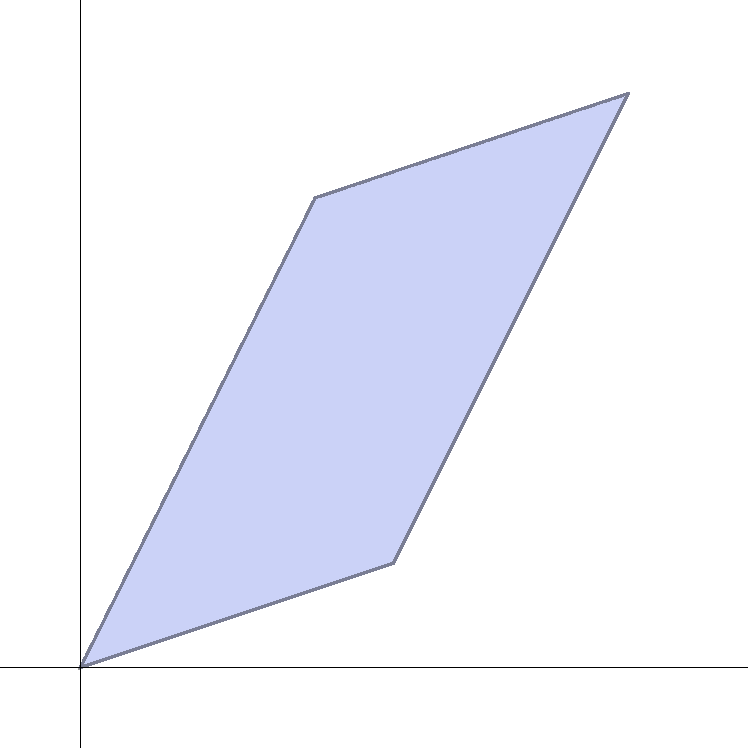
\includegraphics[width = 5truecm]{20150916-fig1.pdf}
\begin{picture}(0,0)
\put(-130.5, 15.3){\vector(1,2){45}}
\put(-130.6, 15.5){\vector(3,1){60}}
\put(-65, 30){$\begin{pmatrix}a \\ c\end{pmatrix}$}
\put(-110, 105){$\begin{pmatrix}b \\ d\end{pmatrix}$}
\end{picture}
\qquad
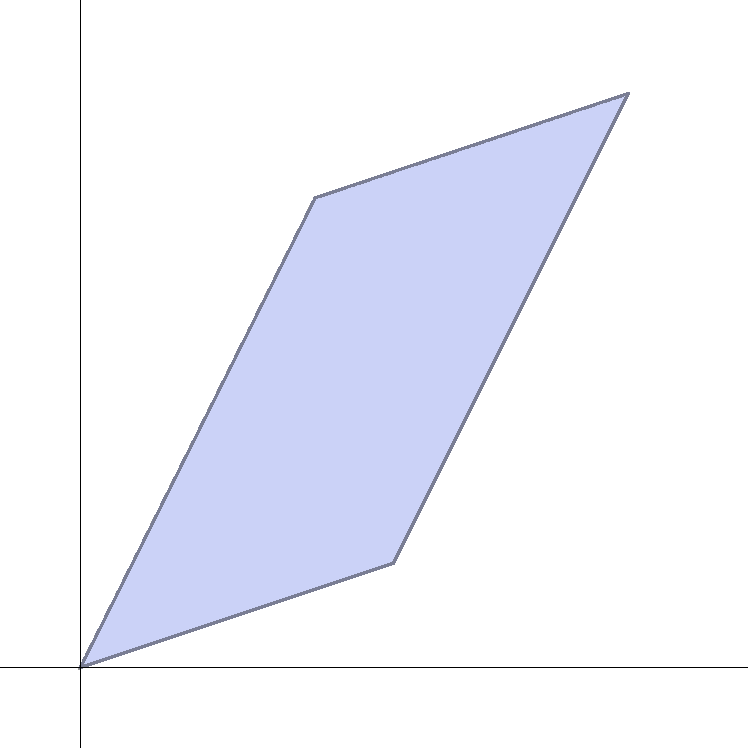
\includegraphics[width = 5truecm]{20150916-fig1.pdf}
\begin{picture}(0,0)
\put(-130.3, 15.6){\dashbox(44.6, 89.2){}}
\put(-130.3, 15.6){\dashbox(59.5, 19.7){}}
\put(-130.3, 15.6){\dashbox(104.1, 109.1){}}
\put(-88, 7.5){$b$}
\put(-73, 8){$a$}
\put(-37.5, 8){$a + b$}
\put(-138, 33){$c$}
\put(-138, 102){$d$}
\put(-154, 122){$c + d$}
\end{picture}
\end{figure}

この図を見れば、面積は
\[
(a + b)(c + d) - \frac{ac}{2} - \frac{bd}{2} - \frac{\bigl(b + (a + b)\bigr)c}{2} - \frac{\bigl(c + (c + d)\bigr)b}{2}
= ad - bc
\]
と求まります。確かに行列式になっていますね。

次に行列式の符号を考えてみます。図のように$a, b, c ,d > 0$の状況なら
\[
ad - bc > 0 \Longleftrightarrow \frac{c}{a} < \frac{d}{b}
\]
です。つまりベクトル${}^t(a, c)$の傾きが${}^t(b, d)$の傾きより小さいときに$ad - bc > 0$というわけです。これは「第$1$象限内で${}^t(a, c)$を反時計回りに回すと${}^t(b, d)$の方向になる」ということと同じです。

これ以外の場合の地道にチェックしなければいけませんが、平面内の$2$本のベクトル$\bm{u}, \bm{v} \in \mathbb{R}^2$を並べてできる行列の行列式$\det(\bm{u} \ \bm{v})$は
\begin{itemize}
\item 絶対値が$\bm{u}$と$\bm{v}$の張る平行四辺形の面積
\item 符号は、平行四辺形において$\bm{u}$から$\bm{v}$を見る方向が右回りなら$+$、左回りなら$-$
\end{itemize}
という性質を持っています。

このことを考えれば、$\bm{u}, \bm{v}$が一次独立であることと$\det(\bm{u}\ \bm{v}) \neq 0$が同値なのは一目瞭然でしょう。$\det(\bm{u}\  \bm{v}) = 0$は「$\bm{u}$と$\bm{v}$の張る平行四辺形の面積が$0$になること」と同値です。この条件は「$\bm{u}$と$\bm{v}$が同じ向きを向いていること」つまり$\bm{u}$と$\bm{v}$が$1$次従属なことに他なりません。僕たちは後に一般の次元で、$\det A \neq 0$と$A$の正則性が同値なことを証明します。その際に大事なのは、やはり「符号つき面積」というイメージです。また多重積分で置換積分をする際に「Jacobi行列」というものの行列式が登場します。この証明をするときにも、$\det$が体積を表すという事実は本質的です。今の話をきちんと理解してください。

\paragraph{問5の解答} 連立$1$次方程式
\begin{align*}
ax + by &= e \\
cx + dy &= f
\end{align*}
に対し、$d\times\text{第1式} - b\times\text{第2式}$, $a\times\text{第2式} - c\times\text{第1式}$を計算すると
\begin{align*}
(ad - bc)x = ed - cf, (ad - bc)y = af - eb
\end{align*}
を得る。これを行列式で書きなおすと
\begin{align*}
x = 
\det
\begin{pmatrix}
e & b \\
f & d
\end{pmatrix}
/
\det
\begin{pmatrix}
a & b \\
c & d
\end{pmatrix}, 
y =
\det
\begin{pmatrix}
a & e \\
c & f
\end{pmatrix}
/
\det
\begin{pmatrix}
a & b \\
c & d
\end{pmatrix}
\end{align*}
となる。

\paragraph{Cramerの公式} こんな感じで、$2$本の方程式からなる$2$変数の$1$次方程式の解が行列式で表せました。より一般に、変数と方程式の本数が一致している連立$1$次方程式の解が唯一存在するとき、それを行列式で書き下す公式が存在します。それが\textbf{Cramerの公式}と呼ばれるものです。まだ$n$次の行列式を定義していないので、それが終わった後で一般の場合を紹介します。

\subsection{$3$次の行列式}

$3$次の行列式も、まず定義式を書いてみます。
\[
\det
\begin{pmatrix}
a & b & c \\
d & e & f \\
g & h & i
\end{pmatrix}
:=  aei + bfg + chd - ceg - bdi - ahf
\]
この式には$2$つの覚え方があります。$1$つ目は\textbf{Sarrusの方法}と呼ばれるものです。次の図のように、行列式を取る行列と曲がった矢印を重ねます。そして最初右下に向かう矢印はそのまま、左下に向かう矢印にはマイナスの符号をつけて、全て足すのです。

% Sarrus
\begin{figure}[h!tbp]
\centering
\end{figure}

もう$1$つの覚え方は、\textbf{余因子展開}というものです。さっきの行列式をよく見ると
\begin{align*}
\det
\begin{pmatrix}
a & b & c \\
d & e & f \\
g & h & i
\end{pmatrix}
&=  aei + bfg + chd - ceg - bdi - ahf
= a(ei - hf) - b(di - fg) + c(hd - eg) \\
&=
a
\begin{pmatrix}
e & f \\
h & i
\end{pmatrix}
- b
\begin{pmatrix}
d & f \\
g & i
\end{pmatrix}
+ c
\begin{pmatrix}
d & e \\
g & h
\end{pmatrix}
\end{align*}
となっています。ルールが分かるような書き方をすると、こうなります:
\begin{itemize}
\item \uline{$1$}行目と\uline{$1$}列目を取り去ってできる小行列の行列式を、\uline{$(1, 1)$}成分の$a$にかける
\item \uline{$1$}行目と\uline{$2$}列目を取り去ってできる小行列の行列式を、\uline{$(1, 2)$}成分の$b$にかける
\item \uline{$1$}行目と\uline{$3$}列目を取り去ってできる小行列の行列式を、\uline{$(1, 3)$}成分の$c$にかける
\end{itemize}
ということをやって、$\pm$の符号を交互にして足しているのです。要となる成分が$1$行目を左から順に動くので、これを\textbf{$1$行目に関する余因子展開}といいます。

今と同じことを、列に関しても考えられます。行列式の定義式は
\begin{align*}
\det
\begin{pmatrix}
a & b & c \\
d & e & f \\
g & h & i
\end{pmatrix}
&=  aei + bfg + chd - ceg - bdi - ahf
= a(ei - hf) - d(bi - ch) + g(bf - ce) \\
&=
a
\begin{pmatrix}
e & f \\
h & i
\end{pmatrix}
- d
\begin{pmatrix}
b & c \\
h & i
\end{pmatrix}
+ g
\begin{pmatrix}
b & c \\
e & f
\end{pmatrix}
\end{align*}
と書き直せます。この式は
\begin{itemize}
\item \uline{$1$}行目と\uline{$1$}列目を取り去ってできる小行列の行列式を、\uline{$(1, 1)$}成分の$a$にかける
\item \uline{$2$}行目と\uline{$1$}列目を取り去ってできる小行列の行列式を、\uline{$(2, 1)$}成分の$b$にかける
\item \uline{$3$}行目と\uline{$1$}列目を取り去ってできる小行列の行列式を、\uline{$(3, 1)$}成分の$c$にかける
\end{itemize}
ということをやって、出てくる数に$\pm$を交互につけて足しています。こっちは要となる成分が$1$列目を縦に動くので、\textbf{$1$列目に関する余因子展開}といいます。同じようにして$i$行目あるいは$j$列目に関する余因子展開をすることもできますが、まずは$1$行目 / $1$列目での余因子展開を確実にできるようになりましょう。これさえできれば、行 / 列を動かしてもやることは同じです。

\paragraph{問4 (1) の解答} 定義通りに計算すれば、次を得る。
\[
D_2 = \det
\begin{pmatrix}
t & 1 \\
1 & t
\end{pmatrix}
= t^2 - 1, \quad
D_3 = \det
\begin{pmatrix}
t & 1 & 0 \\
1 & t & 1 \\
0 & 1 & t
\end{pmatrix}
= t^3 - 2t
\]
\qed

\paragraph{問2 (1), (4) の解答} 定義通りに計算すれば、次を得る。
\[
\det
\begin{pmatrix}
1 & 2 & 3 \\
2 & 3 & 4 \\
3 & 4 & 5
\end{pmatrix}
= 0, \quad
\begin{pmatrix}
1 & a & a^2 \\
1 & b & b^2 \\
1 & c & c^2
\end{pmatrix}
= (b - a)(c - a)(c - b)
\]
\qed

\paragraph{Vandermonde行列式} ここで出てきた (4) の行列式は ($3$次の) \textbf{Vandermonde行列式}と呼ばれます\footnote{今はこの名前で定着していますが、実のところはVandermonde自身とそこまで深い関係にはないようです。この名前がついた詳しい歴史が \url{http://arxiv.org/abs/1204.4716} に載っています。}。また、Vandermonde行列式の値$(b - a)(c - a)(c - b)$は$a, b, c$の\textbf{差積}と呼ばれます。$a, b, c$から$2$つを選ぶ全ての組合せについて差を計算し、その積を取っているから、差積という名前がついています。

この「Vandermonde行列式$=$差積」という式は非常に重要です。というのも差積は
\begin{itemize}
\item 差積が$0$にならないことと$a, b, c$が相異なることが同値
\item $a, b, c$の交代式は必ず差積で割り切れる
\end{itemize}
という性質を持っているからです。一方でVandermonde行列式の中身を係数行列に持つような連立一次方程式を解きたい場面が、この後たまに出てきます。そういう時に計算結果を知っていれば、方程式の解が存在するかどうか、直ちに判定することができます。

\section{4次以上の行列式}

\subsection{高次の行列式の計算法}

$4$次より大きい行列式に対しても、やることは同じです。高次の行列式は、余因子展開で計算することができます。たとえば$4$次の行列式の場合
\begin{align*}
&\det
\begin{pmatrix}
a_{11} & a_{12} & a_{13} & a_{14} \\
a_{21} & a_{22} & a_{23} & a_{24} \\
a_{31} & a_{32} & a_{33} & a_{34} \\
a_{41} & a_{42} & a_{43} & a_{44}
\end{pmatrix} \\
&= a_{11} \det
\begin{pmatrix}
a_{22} & a_{23} & a_{24} \\
a_{32} & a_{33} & a_{34} \\
a_{42} & a_{43} & a_{44}
\end{pmatrix}
- a_{12} \det
\begin{pmatrix}
a_{21} & a_{23} & a_{24} \\
a_{31} & a_{33} & a_{34} \\
a_{41} & a_{43} & a_{44}
\end{pmatrix}
+ a_{13} \det
\begin{pmatrix}
a_{21} & a_{22} & a_{24} \\
a_{31} & a_{32} & a_{34} \\
a_{41} & a_{42} & a_{44}
\end{pmatrix}
- a_{14} \det
\begin{pmatrix}
a_{21} & a_{22} & a_{23} \\
a_{31} & a_{32} & a_{33} \\
a_{41} & a_{42} & a_{43}
\end{pmatrix}
\end{align*}
という式が成り立ちます。一般に$n$次の行列式は余因子展開によって$n - 1$次の行列式の計算に帰着できます。これを使えば、再帰的に行列式の計算を$2$次まで落としこめるというわけです\footnote{行列式には
\begin{itemize}
\item このプリントに書いた、置換に関する$\sum$で定義する式
\item 「交代性」および「多重線型性」というものを用いる定義
\end{itemize}
という$2$種類の定義があり、どちらを採用しても同じ結果が得られることが知られています。どちらの定義も一長一短あるのですが、今回僕たちは前者の定義を採用して話を進めるので、余因子展開は最終的に「定義」ではなく「定理」として得られます。}。後で余因子展開の式が正しいことを証明しますが、証明は脇に置いといて、今回は使い方を見てみましょう。

\paragraph{問2 (2), (3), (5) の解答} (2) $-3$ \quad (3) $12$ \quad (5) $(ad - bc)^2$

\paragraph{問4 (2) の解答} $D_n$の$\det$の中身を
\begin{align*}
A_n := 
\begin{pmatrix}
t & 1 & 0 & \cdots & 0 \\
1 & t & 1 & \ddots & \vdots \\
0 & 1 & t & \ddots & 0 \\
\vdots & \ddots & \ddots & \ddots & 1 \\
0 & \cdots & 0 & 1 & t
\end{pmatrix}
\end{align*}
とおく。この式を$1$行目について余因子展開すると
\[
D_n = \det A_n
= t \det A_{n - 1} + 1 \det
\begin{pmatrix}
1 & * \\
\bm{0} & A_{n - 2} \\
\end{pmatrix}
\]
となる\footnote{行列式の計算に寄与しないどうでもいい部分を$*$で表しました。}。第$2$項は$1$列目に関して余因子展開すると$D_{n - 2} = \det A_{n - 2}$となるから、結局$D_n = t D_{n - 1} + D_{n - 2}$という漸化式が得られる。これによって
\begin{align*}
D_t &=
t D_4 - D_3 = t(t D_3 - D_2) - D_3 = (t^2 - 1) - t D_2 \\
&= (t^2 - 1)(t^3 - 2t) - t(t^2 - 1) = (t^2 - 1)(t^3 - 3t)
\end{align*}
を得る。\qed

\subsection{特別な形の行列式}

\paragraph{問3 (1) の解答} $1$列目に関する余因子展開を繰り返すことで
\[
\det
\begin{pmatrix}
1 & 5 & 8 & 10 \\
0 & 2 & 6 & 9 \\
0 & 0 & 3 & 7 \\
0 & 0 & 0 & 4
\end{pmatrix}
= 1 \det
\begin{pmatrix}
2 & 6 & 9 \\
0 & 3 & 7 \\
0 & 0 & 4
\end{pmatrix}
= 2 \det
\begin{pmatrix}
3 & 7 \\
0 & 4
\end{pmatrix}
= 24
\]
を得る。 \qed

\paragraph{三角行列の行列式}
今の式変形を見れば分かると思いますが、上三角行列の行列式は、対角成分を全て掛け算すれば得られます。理由は簡単で、
\begin{itemize}
\item $1$行目に関する余因子展開をすると、$0$でない項が$1$個しか現れない
\item 生き残る項に現れる行列式も、また上三角行列の行列式になっている
\end{itemize}
という事情があるからです。下三角行列の場合も、$1$列目に関する余因子展開を繰り返せば同じ結果が得られます。

\paragraph{問3 (2) の解答} $1$列目について余因子展開すると
\[
\det
\begin{pmatrix}
1 & 5 & 8 & 10 \\
a & 2 & 6 & 9 \\
0 & 0 & 3 & 7 \\
0 & 0 & 0 & 4
\end{pmatrix}
= 1 \det
\begin{pmatrix}
2 & 6 & 9 \\
0 & 3 & 7 \\
0 & 0 & 4
\end{pmatrix}
- a
\begin{pmatrix}
5 & 8 & 10 \\
0 & 3 & 7 \\
0 & 0 & 4
\end{pmatrix}
= 24 - 60a
\]
を得る。 \qed

\paragraph{多項式の行列式}

今回の問3 (2) や問4では、多項式を成分とする正方行列が登場します。このような場合、行列式の値も多項式になります。さらに\textbf{行列式の値を取る前と後のどっちで変数に値を代入しても、出てくる結果は同じ}です。というのも行列式は定義式が多少ややこしいものの、所詮は成分を適当に掛け算して足し合わせるだけに過ぎません。一方で任意の多項式$f(x), g(x) \in \mathbb{R}[x]$に対し、$h(x) := f(x)g(x)$とおけば、全ての$a \in \mathbb{R}$について$h(a) = f(a)g(a)$が成り立ちます。多項式について掛け算と代入の順序が入れ替えられることから、行列式についても掛け算と数の代入の順序が入れ替えられます。

これを知っていれば、たとえば問3 (2) は「$a = 0$を代入したときに (1) と同じ値になるかどうか」で検算ができます。あるいは「最初に (2) を解いて、その結果に$a = 0$を代入したものが (1) の答えになる」という手抜きもできます。今回は上三角行列の行列式だから手抜きをするほどのこともないですが、このテクニックは覚えておいて損はしません。

\section{置換と$n$次対称群}

行列式の定義式をもう一度見直してみましょう。$n$次の正方行列$A = (a_{ij})_{1 \leq i, j \leq n}$の行列式は
\[
\det A = \sum_{\sigma \in \mathfrak{S}_n} \sgn(\sigma) a_{1 \sigma(1)} a_{2 \sigma(2)} \cdots a_{n \sigma(n)}
\]
という式で定義されています。この式の$\sum_{\sigma \in \mathfrak{S}_n}$は「集合$\mathfrak{S}_n$の全ての元$\sigma$にわたって和を取る」という意味なので、行列式を理解するには``$\mathfrak{S}_n$''が何だか分からないと、話が進みません。また$\sgn(\sigma)$という記号も、まだ定義していません。この式が読めるようになるよう、「$n$次対称群$\mathfrak{S}_n$」について調べてみましょう。

\subsection{置換の定義}

\paragraph{定義}

天下りですが、まず定義を与えてしまいましょう。$1, 2, \ldots, n$を並べ替える写像を、$\{1, 2, \ldots, n\}$の\textbf{置換}といいます。たとえば$n = 3$なら
\[
\sigma(1) = 3, \quad \sigma(2) = 1, \quad \sigma(3) = 2
\]
で定まる写像が$\{1, 2, 3\}$の置換です。$\sigma$に$1, 2, 3$を放り込むと、それぞれの値として$3, 1, 2$が出てきます。これは$1, 2, 3$の並び替えになっていますね。他にもたとえば
\[
\tau(2) = 1, \quad \tau(2) = 3, \quad \tau(3) = 2
\]
も$\{1, 2, 3\}$の置換です。$1, 2, 3$を並べ替える方法は全部で$6$通りですから、上に挙げた他にも$4$つの置換があります。

もう少し写像としての見方を強調するなら、$1, 2, 3$の並べ替えとは「値として$1, 2, 3$がちょうど$1$度ずつ現れるような写像$\{1, 2, 3\}\rightarrow \{1, 2, 3\}$」に他なりません。つまり\textbf{$1, 2, 3$の置換とは、集合$\{1, 2, 3\}$上の全単射}です。

\paragraph{$n$次対称群}
いま定義した$\{1, 2, \ldots, n\}$の置換全てを集めてできる集合を\textbf{$n$次対称群}\footnote{「群」という言葉の意味は、後で説明します。今は気にしないでいいです。}といい、$\mathfrak{S}_n$と書きます。

この見慣れない記号`$\mathfrak{S}$'は、フラクトゥール体 (ドイツ文字) でのアルファベット`S'です。やたら飾りがでかいので、初見では「これのどこがSだよ!」と感じることでしょう。でも手書きにしてみると、中にSが入っているのが分かると思います\footnote{と言ってはみたものの、苦しい言い訳にしか聞こえないですよね……}。
\begin{figure}[h!tbp]
\centering
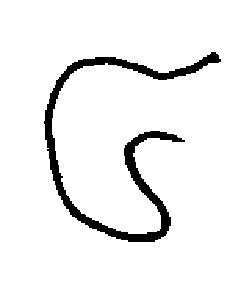
\includegraphics[width = 2truecm]{fraktur_S.pdf}
\qquad\qquad
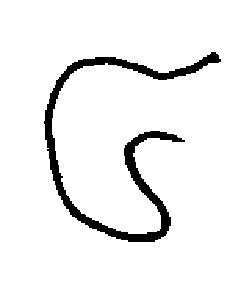
\includegraphics[width = 2truecm]{fraktur_S.pdf}
\begin{picture}(0,0)
\put(-25, 21){\circle{29}}
\put(13, 20){\vector(-1, 0){20}}
\put(13, 17){このへんがS}
\end{picture}
\caption{手書きの`$\mathfrak{S}$'}
\end{figure}

本によっては$\mathfrak{S}_n$の代わりに$S_n$という記号を使っていることもあります。ですから皆さんが「$n$次対称群の記号には$S_n$を使うんだ」と心の中で決心するなら、別に$S_n$と書いても何も問題ありません。ただ$\mathfrak{S}$という記号を使うことにしておくと、$\mathfrak{S}$という文字を見た瞬間に「対称群だ!」と気づくことができます。そういうささやかなメリットがあるからか、対称群を表すのに$\mathfrak{S}$を使う伝統があるので、このプリントでも$\mathfrak{S}$を使うことにします。

ちなみに英語に筆記体があるように、ドイツ語にも (英語とは異なる) 筆記体があります。かつて東大にいらした数学者の岩堀長慶先生\footnote{植野先生の師匠です。残念ながら、2011年にご逝去されました。}は「`$\mathfrak{S}$'はあくまで印刷用の字体であるから、手書きでSを書く時はドイツ語の筆記体のSを使うべきだ」とおっしゃっていたそうです\footnote{このお話は、東大数理科学研究科の寺田至先生に伺いました。寺田先生の師匠も岩堀先生です。}。こだわりたい人は、ドイツ語の筆記体を使ってみても良いでしょう\footnote{たとえば林エルケ『(ドイツ語の本の名前)』に書いてあります。}。ただ残念ながらドイツ語の筆記体が読める人は (少なくとも、日本人の数学者には) あまりいないので、レポートや試験で使う時は断りを入れてください。

\paragraph{あみだくじ}

\subsection{置換の表記}

さて、$n$次の置換$\sigma$は$\sigma\colon \{1, 2, \ldots, n\} \rightarrow \{1, 2, \ldots, n\}$という写像を与えています。したがって「$\sigma$がどんな写像であるか」を記述するには、$1, 2, \ldots, n$の行き先$\sigma(1), \sigma(2), \ldots, \sigma(n)$を全て書く必要があります。この表記法にはいくつかよく使われるものがあるので、それをまとめておきます。

\paragraph{行列記法}

集合$\{1, 2, \ldots, n\}$の置換$\sigma$を表すのに、「上の行に入力、下の行に出力」を並べた$2\times n$の行列を使うことができます。たとえば$n = 3$で$\sigma(1) = 3, \sigma(2) = 1, \sigma(3) = 2$のときは
\[
\sigma =
\begin{pmatrix}
1 & 2 & 3 \\
3 & 1 & 2
\end{pmatrix}
\]
といった感じです。より一般の場合も
\[
\sigma =
\begin{pmatrix}
1 & 2 & \cdots & n \\
\sigma(1) & \sigma(2) & \cdots & \sigma(n)
\end{pmatrix}
\]
というルールにのっとって$\sigma$の行先を並べれば、$\sigma$がどんな写像なのかが分かります。最もよく使われる記法なので、意味をちゃんと抑えておいてください。

また「上の行き先が下」というルールがあるので、$1$行目が$1, 2, \ldots, n$の順番に並ぶ必要はありません。たとえば
\[
\begin{pmatrix}
1 & 2 & 3 \\
3 & 1 & 2
\end{pmatrix}
=
\begin{pmatrix}
3 & 2 & 1 \\
2 & 1 & 3
\end{pmatrix}
\]
といった書き方もできます。積極的に順番を乱す理由はないですが、後で逆置換を考えるときなどは、この記法が役に立ちます。

\paragraph{互換}

さて行列記法はどんな置換でも表せるものの、しばしば無駄が多いです。その際たる例は「$2$つ数だけを入れ替え、他はそのままにする」という置換です。ほとんどの数がそのままにされるなら、省略したいと思うのが自然でしょう。そこで$i \neq j$のとき、「$i$と$j$を入れ替え、他は何もしない」というルールで定まる置換を$(i\ j)$と書きます。たとえば$n = 5$のとき
\[
(2\ 5) =
\begin{pmatrix}
1 & 2 & 3 & 4 & 5 \\
1 & 5 & 3 & 4 & 2
\end{pmatrix}
\]
といった具合です。このように$(i\ j)$の形で書ける置換を\textbf{互換}といい、特に$j = i + 1$のとき、$(i\ i+1)$を\textbf{隣接互換}といいます。

\paragraph{巡回置換} 互換は「$2$つの数を入れ替える」という置換でしたが、これをもう少し拡張した「$n$個の数を順繰りに入れ替える置換」というのも良く使います。このような置換を\textbf{巡回置換}といいます。

巡回置換は、順繰りに入れ替わる数を$1$列に並べて表示します。たとえば$n = 4$で
\[
\sigma =
\begin{pmatrix}
1 & 2 & 3 & 4 \\
4 & 3 & 1 & 2
\end{pmatrix}
\]
の場合、$1$に$\sigma$を繰り返し施すと$1 \rightarrow 4 \rightarrow 2 \rightarrow 3 \rightarrow 1$という順番で数が動きます。そこでこの$\sigma$を$\sigma = (1423)$と書き表します。また$\sigma$を当てると数の列が巡回するので、$1$から書き始める必要もありません。$(1423) = (4231) = (2314) = (3142)$です。巡回置換に現れる数が$2$個のときは、巡回置換は互換になります。

なお、全ての置換が巡回置換の形で書けるわけではありません。たとえば
\[
\sigma = 
\begin{pmatrix}
1 & 2 & 3 & 4 \\
2 & 1 & 4 & 3
\end{pmatrix}
\]
を何回か$1, 2, 3, 4$に施すと、$1 \rightarrow 2 \rightarrow 1$, $3 \rightarrow 4 \rightarrow 3$という$2$つのサイクルがあることに気づきます。後で見るように、一般の場合でも置換を何個かの巡回置換に分解することができます。

\subsection{置換の積}

さて、置換が$2$つあったときに、それらの「積」を定義することができます。それを説明します。

$\sigma, \tau \in \mathfrak{S}_n$とします。このとき$\sigma, \tau$は共に$\{1, \ldots, n\}\rightarrow\{1, \ldots, n\}$という写像なので、合成写像$\sigma \circ \tau \colon \{1, \ldots, n\} \rightarrow \{1, \ldots, n\}$を考えることができます。そこで$\sigma\tau := \sigma \circ \tau$を$\sigma$と$\tau$の\textbf{積}と定めます\footnote{なんでこれが「積」と呼ぶにふさわしいかは、次回説明します。}。

% 逆向きに定義するべき?

一つ例を見てみましょう。たとえば$n = 4$で
\[
\sigma = 
\begin{pmatrix}
1 & 2 & 3 & 4 \\
4 & 2 & 3 & 1
\end{pmatrix}, \quad
\tau = 
\begin{pmatrix}
1 & 2 & 3 & 4 \\
3 & 1 & 2 & 4
\end{pmatrix}
\]
とします。このとき
\begin{align*}
\sigma\bigl(\tau(1)\bigr) &= \sigma(3) = 3 &\sigma\bigl(\tau(2)\bigr) &= \sigma(1) = 4 &\sigma\bigl(\tau(3)\bigr) &= \sigma(2) = 2,
&\sigma\bigl(\tau(4)\bigr) &= \sigma(4) = 1
\end{align*}
だから
\[
\sigma \tau =
\begin{pmatrix}
1 & 2 & 3 & 4 \\
3 & 4 & 2 & 1
\end{pmatrix}
\]
という具合です。なお積を定義するにあたっては「$\mathfrak{S}_n$の元が全単射」という事実が大事です。$\sigma, \tau$は共に全単射なので、合成$\sigma \circ \tau$も全単射で、したがって$\mathfrak{S}_n$の元となります。具体例だと気づきにくいですが、どんな$\sigma, \tau \in \mathfrak{S}_n$を取ってきても$\sigma\tau \in \mathfrak{S}_n$となることは、全単射という性質が保証してくれるのです。

\paragraph{互換による表示}

置換の中である意味最も簡単なのが、$2$個の数を入れ替える互換です。あらゆる置換は、互換の積で表すことができます。たとえば
\[
\begin{pmatrix}
1 & 2 & 3 & 4 \\
4 & 2 & 1 & 3
\end{pmatrix}
= 
\begin{pmatrix}
1 & 2 & 3 & 4 \\
3 & 2 & 1 & 4
\end{pmatrix}
\begin{pmatrix}
1 & 4
\end{pmatrix}
=
\begin{pmatrix}
1 & 2 & 3 & 4 \\
1 & 2 & 3 & 4 \\
\end{pmatrix}
\begin{pmatrix}
1 & 3
\end{pmatrix}
\begin{pmatrix}
1 & 4
\end{pmatrix}
=
\begin{pmatrix}
1 & 3
\end{pmatrix}
\begin{pmatrix}
1 & 4
\end{pmatrix}
\]
といった具合です。今の式変形を見れば分かるように、一般に$\sigma \in \mathfrak{S}_n$に対して互換$(i\ j)$を右からかけると、$\sigma(i)$と$\sigma(j)$の値を入れ替えることができます。したがって、$\sigma$を行列表示したときに
\begin{itemize}
\item 右からうまく互換をかけて、$\sigma$の下の行で$n$を一番右に持っていく
\item 右からうまく互換をかけて、$\sigma$の下の行で$n - 1$を右から$2$番目に持っていく
\item ……
\end{itemize}
という操作をすれば、最終的に$\sigma$を恒等置換に変形することができます。この式を見れば$\sigma$を互換の積に表す式が得られている、というわけです。上に書いた例も同じ手順で式変形をしています。確認してください。

また$i < j$のとき
\[
\begin{pmatrix}
i & j 
\end{pmatrix}
=
\begin{pmatrix}
i & i + 1
\end{pmatrix}
\begin{pmatrix}
i + 1 & i + 2
\end{pmatrix}
\cdots
\begin{pmatrix}
j - 2 & j - 1
\end{pmatrix}
\begin{pmatrix}
j - 1 & j
\end{pmatrix}
\begin{pmatrix}
j - 2 & j - 1
\end{pmatrix}
\begin{pmatrix}
j - 3 & j - 2
\end{pmatrix}
\cdots
\begin{pmatrix}
i & i + 1
\end{pmatrix}
\]
という式が成り立ちます。何をやっているのかと思うかもしれませんが、あみだくじで書いてみれば一発で分かります。次のあみだくじを辿って、左端から出発したら右端に、右端から出発したら左端にたどり着き、そして他の場所から出発したら真下にたどり着くことを確認してください。
\begin{figure}[h!tbp]
\centering
\begin{picture}(120, 120)
\put(8, 113){$i$}
\put(108, 114){$j$}
\put(10, 10){\line(0, 1){100}}
\put(30, 10){\line(0, 1){100}}
\put(50, 10){\line(0, 1){100}}
\put(70, 10){\line(0, 1){100}}
\put(90, 10){\line(0, 1){100}}
\put(110, 10){\line(0, 1){100}}
\put(10, 20){\line(1, 0){20}}
\put(30, 30){\line(1, 0){20}}
\put(50, 40){\line(1, 0){20}}
\put(70, 50){\line(1, 0){20}}
\put(90, 60){\line(1, 0){20}}
\put(70, 70){\line(1, 0){20}}
\put(50, 80){\line(1, 0){20}}
\put(30, 90){\line(1, 0){20}}
\put(10, 100){\line(1, 0){20}}
\end{picture}
\end{figure}

結局
\begin{itemize}
\item 全ての置換が互換の積で表せる
\item 全ての互換は隣接互換の積で表せる
\end{itemize}
ことが分かったので、\textbf{全ての置換は隣接互換の積で表せる}ことが言えました\footnote{平たく言えば、「隣り合う縦線の間に横線を引く」という操作を使うだけで、どんな並びのあみだくじも作れるということです。}。

\subsection{逆置換}

$\{1, 2, \ldots, n\}$の置換$\sigma \in \mathfrak{S}_n$が与えられると、$1, 2, \ldots, n$のそれぞれに$\sigma(1), \sigma(2), \ldots, \sigma(n)$という数が対応します。この$\sigma(1), \sigma(2), \ldots, \sigma(n)$という数の並びには$1, 2, \ldots, n$がちょうど$1$回ずつ登場するのでした。そこで「各$\sigma(i)$に対して$i$を対応させる」という方法を考えることで、別の置換を作ることができます\footnote{要は、全単射$\sigma$の逆写像を考えるということです。}。これを$\sigma$の\textbf{逆置換}といい、$\sigma^{-1}$で表します。

あみだくじで見れば、$\sigma^{-1}$を表すのは簡単です。$\sigma$が表すあみだくじの上下をひっくり返したものが、$\sigma^{-1}$に他なりません。

\subsection{置換の符号}

置換は互換の積で表せると言いましたが、その表し方は一通りではありません。たとえば
\[
\begin{pmatrix}
1 & 3
\end{pmatrix}
=
\begin{pmatrix}
1 & 2
\end{pmatrix}
\begin{pmatrix}
2 & 3
\end{pmatrix}
\begin{pmatrix}
1 & 2
\end{pmatrix}
=
\begin{pmatrix}
2 & 3
\end{pmatrix}
\begin{pmatrix}
1 & 2
\end{pmatrix}
\begin{pmatrix}
2 & 3
\end{pmatrix}
\]
が成り立ちます。ところが置換を互換の積で表す方法が何通りかあっても、「表すのに必要な互換の個数の偶奇」は常に一致するのです。上の例も確かにそうなっています。一般にそれが正しいことを示しましょう。

%\paragraph{置換の多項式への作用}

この証明に、差積を使います。
\[
\Delta := \prod_{1 \leq i  < j \leq n} (x_j - x_i)
\]
とおきます。この差積$\Delta$と$\{1, 2, \ldots, n\}$の置換$\sigma \in \mathfrak{S}_n$に対し「$\Delta$の中で$x_i$を$x_{\sigma(i)}$へと入れ替えて得られる多項式」を$\sigma\Delta$と表すことにします\footnote{このことを「互換$(p\ q)$を$\Delta$に作用させる」などといいます。}。実はこのとき、$(p\ q)\Delta = -\Delta$が成り立ちます。

この理由を調べるために、$\Delta$に出てくる項を次のように三角形に並べてみます。これを全部かけたものが差積です\footnote{わざと$1$を並べたのには理由があります。後で互換の作用を調べるときに行番号をこのように調節しておくと、話を進めやすいのです。}。
\[
\begin{array}{cccccc}
1 & \\
x_2 - x_1 & 1 \\
x_3 - x_1 & x_3 - x_2 & 1 \\
\vdots & \vdots & \ddots & \ddots \\
\vdots & \vdots & & \ddots & \ddots \\
x_n - x_1 & x_n - x_2 & \cdots & \cdots &  x_n - x_{n - 1} & 1
\end{array} \qquad
\begin{array}{cccccc} % (3 5) をあてる
1 & \\
x_2 - x_1 & 1 \\
x_3 - x_1 & x_3 - x_2 & 1 \\
x_4 - x_1 & x_4 - x_2 & x_4 - x_3 & 1 \\
x_5 - x_1 & x_5 - x_2 & x_5 - x_3 & x_5 - x_4 & 1 \\
x_6 - x_1 & x_6 - x_2 & x_6 - x_3 & x_6 - x_4 & x_6 - x_5 & 1 \\
\end{array}
\]
左側が一般の場合、右側が$n = 6$の例です。さて、これに互換$(p\ q)$を当てた$(p\ q)\Delta$を考えてみます。$(p\ q)$を当てた時に影響を受ける項は\begin{itemize}
\item $x_p - x_k$ ($1 \leq k < p$) の形の項
\item $x_k - x_p$ ($p \leq k < n$) の形の項
\item $x_q - x_k$ ($1 \leq k < q$) の形の項
\item $x_k - x_q$ ($q \leq k < n$) の形の項
\end{itemize}
の$4$種類です。これらの項の中で$x_p$が$x_q$に、$x_q$が$x_p$へと変化します。さっきの三角形に並べた式を見て、どこの項が$(p\ q)$で影響を受けるのかを図にすると、こんな感じになります\footnote{$n = 6, p = 3, q = 5$の例で確認してみてください。}。
\begin{figure}[h!tbp]
\centering
\begin{picture}(150,150)
\put(10, 10){\line(1, 0){120}}
\put(10, 10){\line(0, 1){120}}
\put(15, 134){$1$}
\put(10, 130){\line(1, 0){15}}
\put(25, 130){\line(0, -1){15}}
\put(30, 119){$1$}
\put(25, 115){\line(1, 0){15}}
\put(40, 115){\line(0, -1){15}}
\put(45, 104){$1$}
\put(40, 100){\line(1, 0){15}}
\put(55, 100){\line(0, -1){15}}
\put(60, 89){$1$}
\put(55, 85){\line(1, 0){15}}
\put(70, 85){\line(0, -1){15}}
\put(75, 74){$1$}
\put(70, 70){\line(1, 0){15}}
\put(90, 59){$1$}
\put(85, 70){\line(0, -1){15}}
\put(85, 55){\line(1, 0){15}}
\put(105, 44){$1$}
\put(100, 55){\line(0, -1){15}}
\put(100, 40){\line(1, 0){15}}
\put(120, 29){$1$}
\put(115, 40){\line(0, -1){15}}
\put(115, 25){\line(1, 0){15}}
\put(135, 14){$1$}
\put(130, 25){\line(0, -1){15}}
\put(3, 105){$p$}
\put(10, 115){\line(1, 0){15}}
\put(10, 100){\line(1, 0){30}}
\put(45, 2){$p$}
\put(40, 10){\line(0, 1){90}}
\put(55, 10){\line(0, 1){75}}
\put(3, 60){$q$}
\put(10, 70){\line(1, 0){60}}
\put(10, 55){\line(1, 0){75}}
\put(90, 2){$q$}
\put(85, 10){\line(0, 1){45}}
\put(100, 10){\line(0, 1){30}}
\put(23, 104){\CID{7555}}
\put(23, 59){\CID{7556}}
\put(43, 30){\CID{7557}}
\put(88, 30){\CID{7558}}
\put(43, 80){\CID{7559}}
\put(65, 59){\CID{7560}}
\put(43, 59){\CID{7561}}
\end{picture}
\end{figure}

この式で$x_p$と$x_q$を入れ替えると、項は次のように変化します。
\begin{itemize}
\item \CID{7555}と\CID{7556}が入れ変わる: $x_p - x_k \longleftrightarrow x_q - x_k$ ($1 \leq k < p$)
\item \CID{7557}と\CID{7558}が入れ変わる: $x_k - x_p \longleftrightarrow x_k - x_q$ ($q < k \leq n$)
\item \CID{7559}と\CID{7560}が$(-1)$倍されて入れ替わる: $x_k - x_p \rightarrow -(x_q - x_k)$, $x_q - x_k \rightarrow -(x_k - x_p)$ ($p < k < q$)
\item \CID{7561}の$x_p - x_q$は$x_q - x_p = -(x_p - x_q)$に変化する
\end{itemize}
さらに\CID{7559}および\CID{7560}にある項の数はどちらも$q - p$個で同じですから、全部の項をかけてしまえば、この部分の$-1$倍は打ち消し合います。よって結局、$x_p - x_q$のところから出てくる$-1$倍だけが残り、$(p\ q)\Delta = -\Delta$が従います。

これが分かると、一般の置換$\sigma \in \mathfrak{S}_n$に対しても$\sigma\Delta$が$\pm\Delta$のどちらになるかが計算できます。互換を$1$個当てるごとに$\Delta$が$-1$倍されるのだから、$\sigma$を互換の積で表しておいて、その個数だけ$-1$をかければよいのです。

さて$\sigma \in \mathfrak{S}_n$を$k$個の互換で表す方法と$l$個の互換で表す方法があったとしましょう。$\Delta$に$(p\ q)$を当てると$-1$倍されるので、$k$個の互換を当てれば$(-1)^k\Delta$に、$l$個の互換を当てれば$(-1)^l\Delta$になります。ところがこれらが一致するので、$k$と$l$の偶奇は等しくないといけません。この事実を使って、$\sigma \in \mathfrak{S}_n$が偶数個の互換の積で表されるとき\textbf{偶置換}、奇数個の互換の積で表されるとき\textbf{奇置換}といいます。そして$\sigma$が偶置換のとき$\sgn(\sigma) = 1$、奇置換のとき$\sgn(\sigma) = -1$と定めます。

\paragraph{$\sgn$の乗法性}

$(-1)$を「$\sigma$を表すのに必要な互換の個数」乗したものが$\sgn(\sigma)$というわけです。したがって任意の$\sigma, \tau \in \mathfrak{S}_n$に対して$\sgn(\sigma\tau) = \sgn(\sigma)\sgn(\tau)$が成り立ちます。

\paragraph{問1の解答}

$\sgn(\sigma^9) = \sgn(\sigma)^9$

\subsection{行列式の定義}
ここまでの準備を経て、ようやく$\det$の定義をきちんと読むことができます。$n$次正方行列$A = (a_{ij})_{1 \leq i,j \leq n}$の行列式の定義
\[
\det A := \sum_{\sigma \in \mathfrak{S}_n} \sgn(\sigma) a_{1 \sigma(1)} a_{2 \sigma(2)} \cdots a_{n \sigma(n)}
\]
は「各$\sigma \in \mathfrak{S}_n$に対し$\sgn(\sigma) a_{1 \sigma(1)} a_{2 \sigma(2)} \cdots a_{n \sigma(n)}$を計算し、それを全部足し合わせる」という意味の式です。$n$が小さい場合に、この式に現れる項を書き下してみましょう。

まずは$n = 2$の場合です。$\{1, 2\}$の置換は恒等置換$\id$と互換$(1\ 2)$の$2$つしかありません。$s = (1 \ 2)$と書くことにすると、$\mathfrak{S}_2 = \{\id, s\}$で、かつ$\sgn(\id) = 1$, $\sgn(s) = -1$です。したがって
\[
\sum_{\sigma \in \mathfrak{S}_2} \sgn(\sigma) a_{1 \sigma(1)} a_{2 \sigma(2)}
= \sgn(\id) a_{1 \id(1)} a_{2 \id(2)} + \sgn(s) a_{1 s(1)} a_{2 s(2)} = a_{11} a_{22} - a_{12} a_{21}
\]
となります。これは紛れもなく$2$次の行列式ですね。

次に$n = 3$でやってみます。$\{1, 2, 3\}$を並べ替えるやり方は全部で$6$通りだから、$\mathfrak{S}_3$は$6$個の元からなります。そこで各$\sigma \in \mathfrak{S}_3$について$\sgn(\sigma)$と$\sgn(\sigma) a_{1\sigma(1)} a_{2\sigma(2)} a_{3\sigma(3)}$の表を作ってみます。
\begin{table}[h!tbp]
\centering
\begin{tabular}{c||cccccc} \hline
置換 &
$\begin{pmatrix}
1 & 2 & 3 \\
1 & 2 & 3
\end{pmatrix}$ & 
$\begin{pmatrix}
1 & 2 & 3 \\
2 & 1 & 3
\end{pmatrix}$ & 
$\begin{pmatrix}
1 & 2 & 3 \\
1 & 3 & 2
\end{pmatrix}$ & 
$\begin{pmatrix}
1 & 2 & 3 \\
2 & 3 & 1
\end{pmatrix}$ & 
$\begin{pmatrix}
1 & 2 & 3 \\
3 & 1 & 2
\end{pmatrix}$ & 
$\begin{pmatrix}
1 & 2 & 3 \\
3 & 2 & 1
\end{pmatrix}$ \\ \hline
符号 & $1$ & $-1$ & $-1$ & $1$ & $1$ & $-1$ \\ \hline
対応する項 & $a_{11} a_{22} a_{33}$ & $-a_{12} a_{21} a_{33}$ & $-a_{11} a_{23} a_{32}$ & $a_{12} a_{23} a_{31}$ & $a_{13} a_{21} a_{32}$ & $-a_{13} a_{22} a_{31}$ \\ \hline
\end{tabular}
\end{table}

この式に基づいて$\det$の定義式を書き下してみると
\[
\sum_{\sigma \in \mathfrak{S}_2} \sgn(\sigma) a_{1 \sigma(1)} a_{2 \sigma(2)} a_{3 \sigma(3)}
= a_{11} a_{22} a_{33} - a_{12} a_{21} a_{33} - a_{11} a_{23} a_{32} + a_{12} a_{23} a_{31} + a_{13} a_{21} a_{32} - a_{13} a_{22} a_{31}
\]
となります。Sarrusの方法で計算する行列式と、確かに一致していますね。$n$が$4$以上の場合も同じようにやれば、計算ができるはずです。ただし$n!$個の項が出てきて大変なので、わざわざ書き下してみる必要はありません。「この式で定義ができる」ということが分かれば十分です。

こんな感じで、行列式はきちんと定義するのにも一苦労するわけですが、僕たちはさらに行列式の計算公式を証明しないといけません。次の週は、この定義式をもとに高次の行列式を計算するための様々な公式を導きましょう。

